\begin{tikzpicture}
	\savebox\mygraphic{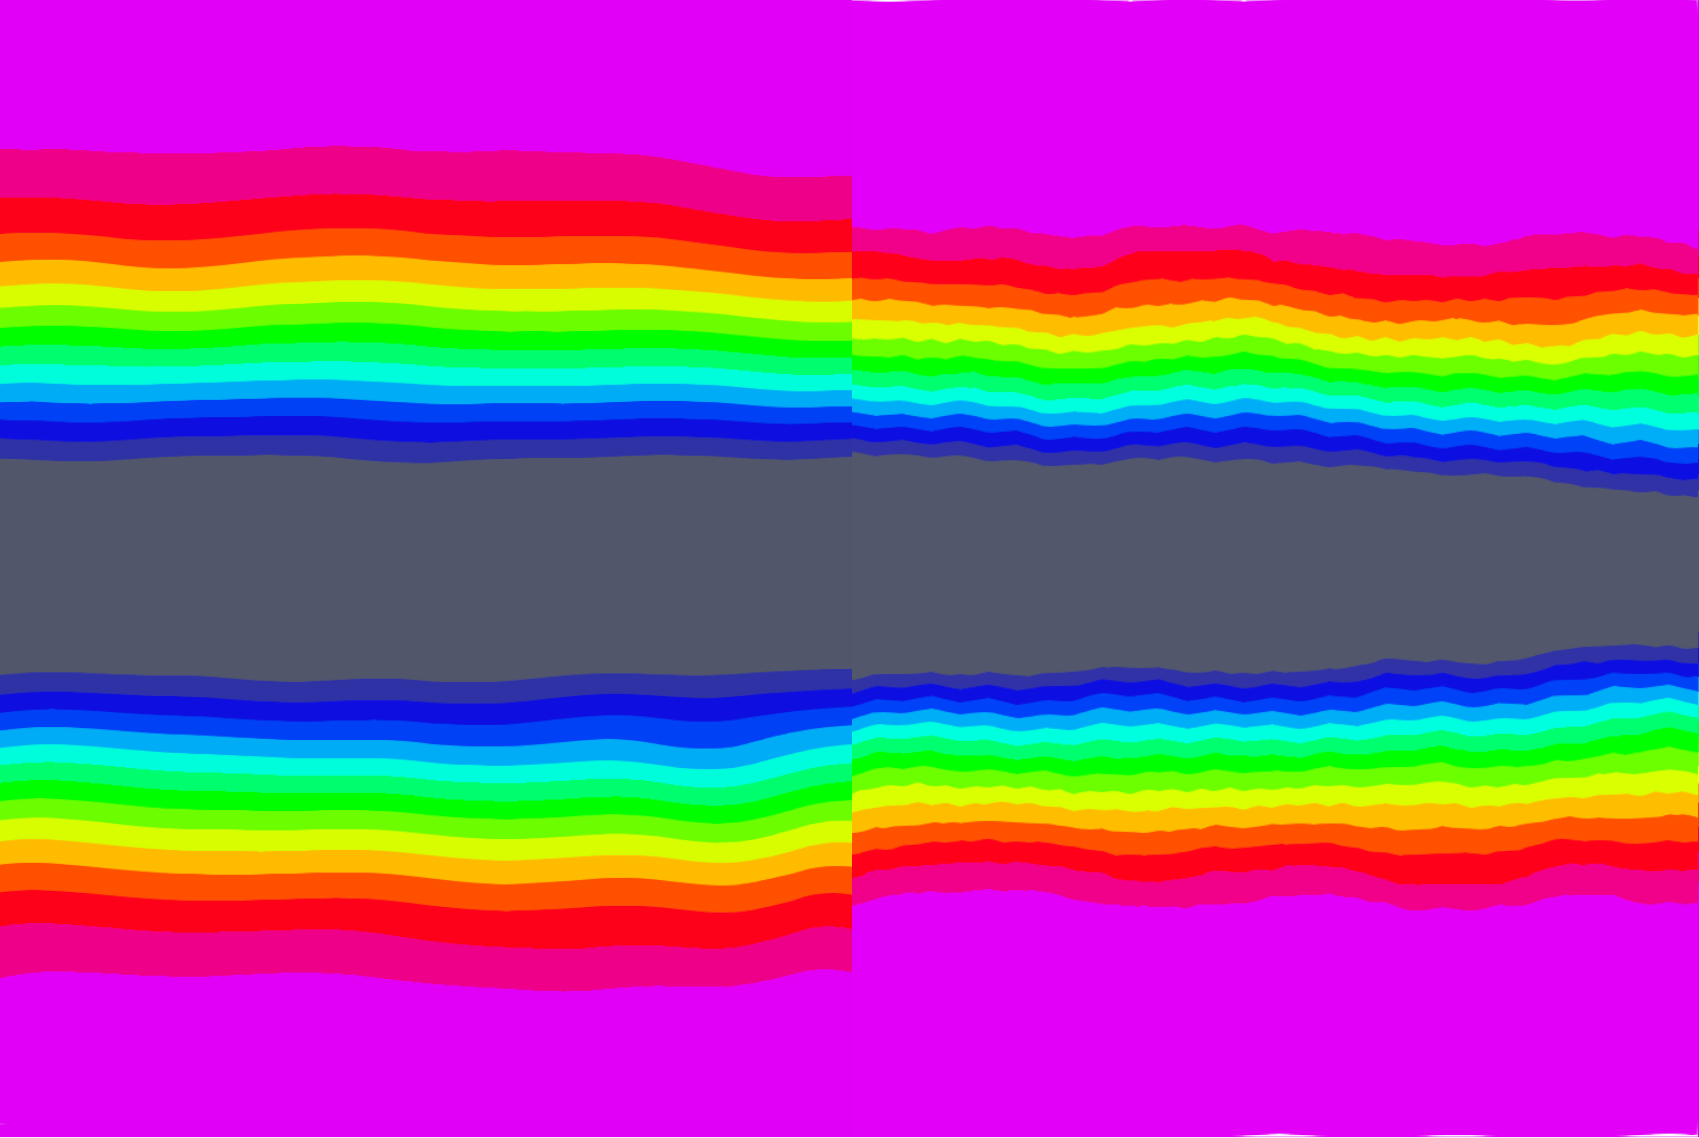
\includegraphics[trim = 0px 0px 0px 0px,clip,width = 0.39\textwidth]{\myImages/res/uXMeanCompPOM2V2.png}}
	\begin{axis}[
		name = plot1,
		xlabel={$z_r$ [--]},
		ylabel={$y_r$ [--]},
		font = \scriptsize,
		xtick distance=1,ytick distance=1,
		width=\wd\mygraphic,
		height=\ht\mygraphic, %height= 5/3*0.5
		enlargelimits=false,
		scale only axis=true,
		tick align=outside,
		ytick pos=left,
		xtick pos=top,
		y label style = {at={(axis cs:-3.6,0)}},
		% x label style = {at={(axis cs:0,-2.7)}},
		line width = 1.7pt
		]
		\addplot graphics[xmin=-3, xmax=3, ymin=-2, ymax=2,includegraphics={trim = 0px 0px 0px 0px,clip}] {\myImages/res/uXMeanCompPOM2V2.png};
		% \fill [white] (axis cs:0.001,-1.997) rectangle (axis cs:0.5,1.997);
		% \fill [black!70](axis cs:0,0) circle [radius=0.5];
		% \draw [black,dashdotted,line width = 1.0pt] (axis cs:-2,0) -- (axis cs:2,0);
		\draw [black!70,dashed,line width = 1.0pt] (axis cs:0,2) -- (axis cs:0,-2);
		\node [white] at (axis cs:0.2,1.7) {\scriptsize{$\zeta$}};
		\node [white] at (axis cs:-2.55,1.75) {\scriptsize{PIV}};
		\node [white] at (axis cs:-2.7,0) {\scriptsize{a)}};
		\node [white] at (axis cs:2.55,1.75) {\scriptsize{CFD}};
	\end{axis}
	\node [name = osaUx,anchor = south east,at={(plot1.south east)},yshift=-0.7cm] {
\includegraphics[width=0.26\textwidth]{\myImages/res/U_x_scale2.png}};
	\node [name = ux, anchor = east,at={(osaUx.north west)},yshift=-0.1cm,xshift=-0.1cm] {\scriptsize{$u_r$ [--]}};
	\node [name = psi0, anchor = south,at={(osaUx.north)},yshift=-0.2cm,xshift=-1.6cm] {\scriptsize{\ 0.7}};
	\node [name = psi0, anchor = west,at={(psi0.east)},xshift=0.45cm] {\scriptsize{0.8}};
	\node [name = psi0, anchor = west,at={(psi0.east)},xshift=0.45cm] {\scriptsize{0.9}};
	\node [name = psi0, anchor = west,at={(psi0.east)},xshift=0.45cm] {\scriptsize{1.0}};
	% \node [name = psi0, anchor = west,at={(psi0.east)},xshift=-0.11cm] {\scriptsize{0.98}};
	% \node [name = psi0, anchor = west,at={(psi0.east)},xshift=-0.14cm] {\scriptsize{1.02}};

	\savebox\mygraphic{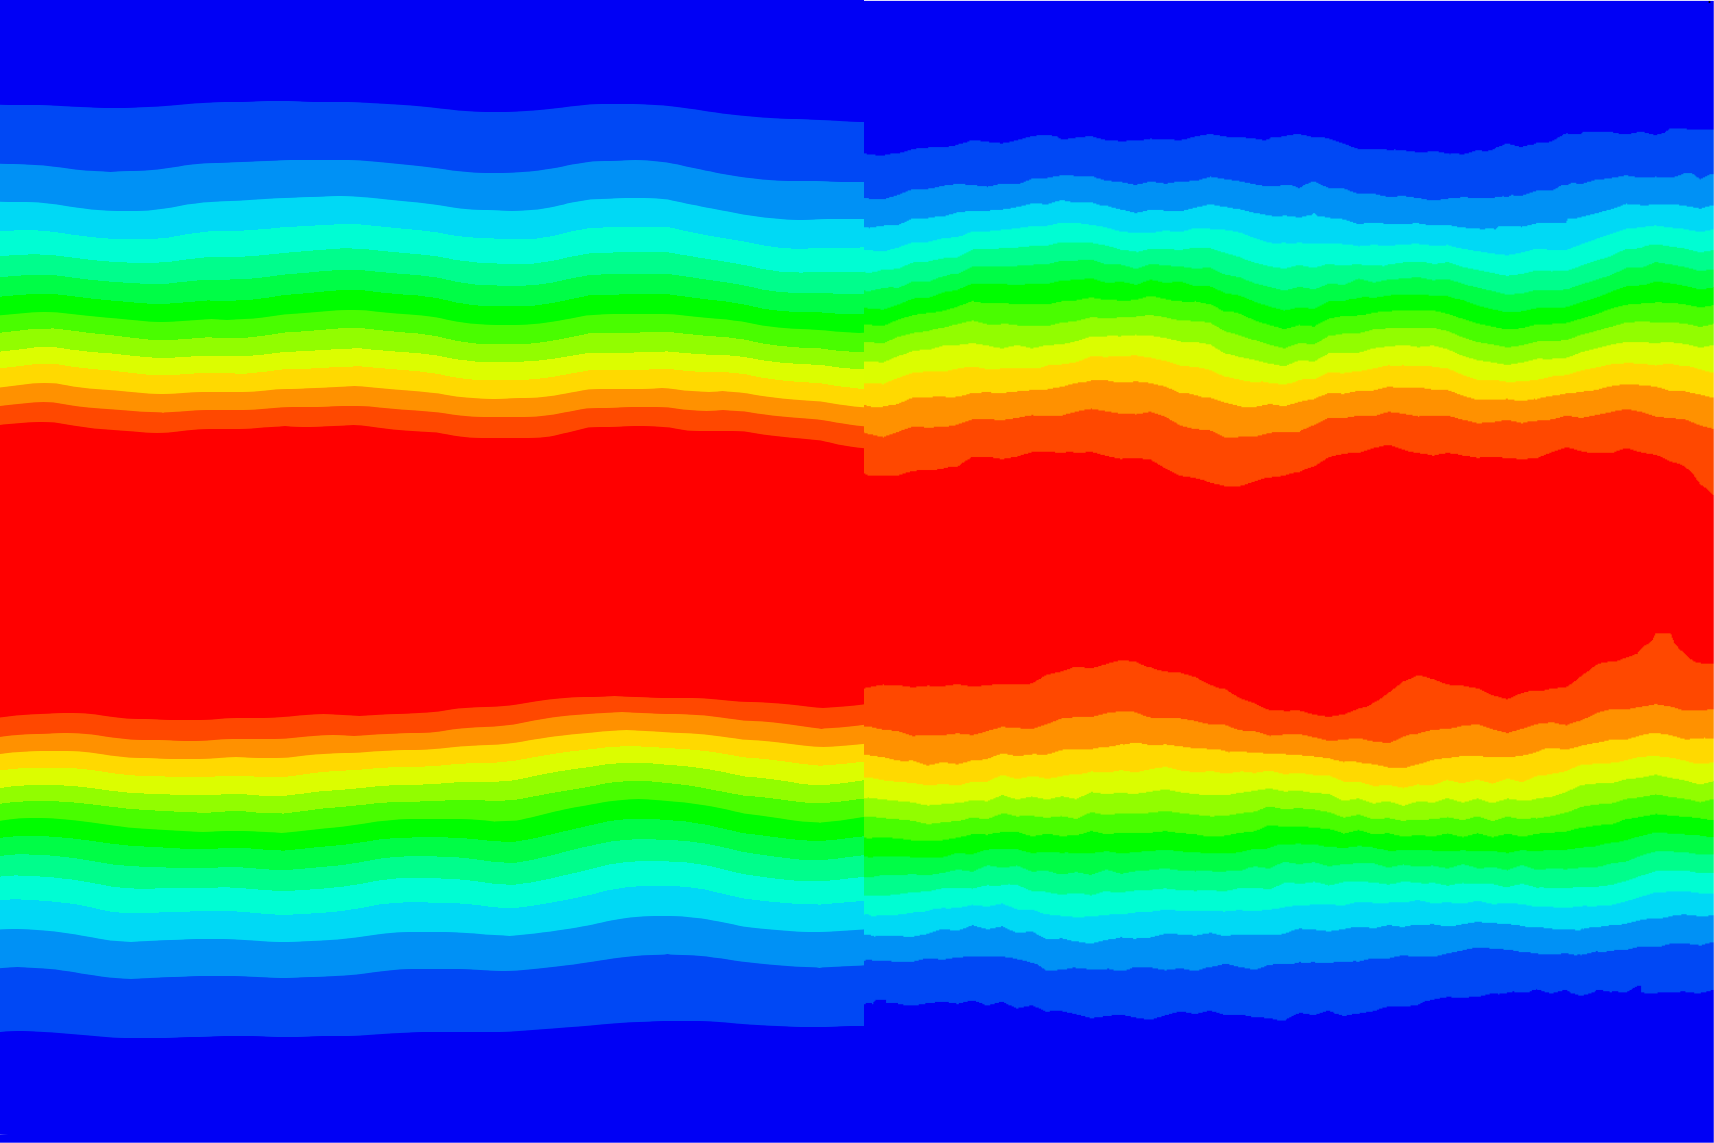
\includegraphics[trim = 0px 0px 0px 0px,clip,width = 0.39\textwidth]{\myImages/res/kMeanCompPOM2.png}}
	\begin{axis}[
		name = plot2,
		anchor = west,
		at = {(plot1.east)},
		xshift = 0.4cm,
		xlabel={$z_r$ [--]},
		ylabel={$y_r$ [--]},
		% x label style = {at={(axis cs:0,-2.7)}},
		y label style = {at={(axis cs:3.5,0)}},
		font = \scriptsize,
		xtick distance=1,ytick distance=1,
		width=\wd\mygraphic,
		height=\ht\mygraphic, %height= 5/3*0.5
		enlargelimits=false,
		scale only axis=true,
		tick align=outside,
		ytick pos=right,
		xtick pos=top,
		line width = 1.7pt
		]
		\addplot graphics[xmin=-3, xmax=3, ymin=-2, ymax=2,includegraphics={trim = 0px 0px 0px 0px,clip}] {\myImages/res/kMeanCompPOM2.png};
		% \fill [white] (axis cs:0.001,-1.997) rectangle (axis cs:0.5,1.997);
		% \fill [black!70](axis cs:0,0) circle [radius=0.5];
		% \draw [black,dashdotted,line width = 1.0pt] (axis cs:-2,0) -- (axis cs:2,0);
		\draw [black!70,dashed,line width = 1.0pt] (axis cs:0,2) -- (axis cs:0,-2);
		\node [white] at (axis cs:0.2,1.7) {\scriptsize{$\zeta$}};
		\node [white] at (axis cs:-2.55,1.75) {\scriptsize{PIV}};
		\node [white] at (axis cs:2.55,1.75) {\scriptsize{CFD}};
		\node [black] at (axis cs:-2.7,0) {\scriptsize{b)}};
	\end{axis}
	\node [name = osak,anchor = south east,at={(plot2.south east)},yshift=-0.7cm,xshift=0.1cm] {
\includegraphics[width=0.26\textwidth]{\myImages/res/k_scale2.png}};
	\node [name = k, anchor = east,at={(osak.north west)},yshift=-0.1cm,xshift=-0.1cm] {\scriptsize{$k$ [--]}};
	\node [name = psi0, anchor = south,at={(osak.north)},yshift=-0.2cm,xshift=-1.49cm] {\scriptsize{0.00}};
	\node [name = psi0, anchor = west,at={(psi0.east)},xshift=0.03cm] {\scriptsize{0.04}};
	\node [name = psi0, anchor = west,at={(psi0.east)},xshift=0.03cm] {\scriptsize{0.08}};
	\node [name = psi0, anchor = west,at={(psi0.east)},xshift=0.03cm] {\scriptsize{0.12}};
	\node [name = psi0, anchor = west,at={(psi0.east)},xshift=0.03cm] {\scriptsize{0.15}};
	% \node [name = psi0, anchor = west,at={(psi0.east)},xshift=-0.2cm] {\scriptsize{0.28}};

	\begin{axis}[
		width=0.815\linewidth,
		height = 3cm,
		yshift = -0.8cm,
		scale only axis,
		name=plot3,
		at = (plot1.south west),
		anchor = north west,
		font = \scriptsize,
		xlabel={$y_{r,\zeta}$ [--]},
		ylabel={$u_r$ [--]},
		% yticklabels={0,0.05,0.1,0.15},
		% yticklabel style={
		% 	/pgf/number format/.cd, fixed, fixed zerofill,
		% 	/pgf/number format/precision=2,
		% 	/pgf/number format/fixed},
		%~ ymode=log,
		%~ xmode=log,
		% ymax = 0.8,
		xmin = -2,
		% ymin = -0.5,
		xmax = 2,
		ytick pos=left,
		mark size=4pt,    
		line width = 0.85pt,
		%~ legend style={at={(axis cs:6,2)},anchor=south west},				
	]
	% \addplot [color = black!50,mark =none]table [y=u_x,x =x]{\myGraphs/msIndData/expLineResV1.dat};\label{expSigm}
	% \addplot [color = blue,mark =none]table [col sep=comma, y expr=(\thisrow{U:0})/5,x expr = {(\thisrow{Points:0})/0.015}]{\myGraphs/msIndData/mS_40p_U.csv};\label{mesh40U}
	% \addplot [color = red,mark =none]table [col sep=comma, y expr=(\thisrow{U:0})/5,x expr = {(\thisrow{Points:0})/0.015}]{\myGraphs/msIndData/mS_50p_U.csv};\label{mesh50U}
	% \addplot [color = green,mark =none]table [col sep=comma, y expr=(\thisrow{U:0})/5,x expr = {(\thisrow{Points:0})/0.015}]{\myGraphs/msIndData/mS_75p_U.csv};\label{mesh70U}
	\addplot [color = blue,mark =none]table [col sep=comma, y expr=(\thisrow{U:0})/5,x expr = {(\thisrow{Points:1})/0.015}]{\myGraphs/msIndData/bCyl_l_3Ver_U.csv};
	\addplot [color = red,mark =none]table [col sep=comma, y expr=(\thisrow{W[m_s]})/5,x expr = {(\thisrow{Points:1}-30.0)/15}]{\myGraphs/msIndData/POM2.csv};
	% \addplot [color = orange,mark =none]table [col sep=comma, y expr=(\thisrow{U:0})/5,x expr = {(\thisrow{Points:0})/0.015}]{\myGraphs/msIndData/mS_120p_U.csv};\label{mesh120U}
	%~ \addplot [color = red,mark =none]table [y=U_x_ms_50_U,x =z_ms_50_U]{\myGraphs/onLineMSV2.dat};\label{mesh50U}
	%~ \addplot [color = green,mark =none]table [y=U_x_ms_70_U,x =z_ms_70_U]{\myGraphs/onLineMSV2.dat};\label{mesh70U}
	%~ \addplot [color = black,mark =none]table [y=U_x_ms_100_U,x =z_ms_100_U]{\myGraphs/onLineMSV2.dat};\label{mesh100U}
	%~ \addplot [color = black,mark =none]table [y=U_x_ms_100_U,x =z_ms_120_U]{\myGraphs/onLineMSV2.dat};\label{mesh100U}
	\coordinate (top) at (rel axis cs:0,1);
	\end{axis}
	\node [name = c, anchor = west,at={(plot3.west)},yshift=-0.0cm,xshift=-0.0cm] {\scriptsize{c)}};
\begin{axis}[
		at = (plot3.north west),
		anchor = north west,
		width=0.815\linewidth,
		height = 3cm,
		scale only axis,
		xlabel={$x_\sigma$ [--]},
		%~ ylabel={\textcolor{red}{TKE}},
		ylabel={$k$ [--]},
		%~height=\figHeight,
		scale only axis,
		%~ xmin=0,
		%~ xmax=600,
		% yticklabels={0,0.05,0.1,0.15},
					yticklabel style={
			/pgf/number format/.cd, fixed, fixed zerofill,
			/pgf/number format/precision=2,
			/pgf/number format/fixed},
		xmin=-2,
		xmax=2,
		ymin=0,
		% ymax = 0.3,
		%~ ymax=1000,
		hide x axis,
		axis y line*=right,
		font=\scriptsize,
		line width = 0.85pt,
		%~ axis line style={red},
		%~ axis y label/.append style ={red},
		%~ ytick label/.append style = {red},
		%~ ylabel={$y_{\mathrm{NO}},\,y_{\mathrm{N_{2}O}} \mathrm{\,[ppm]}$},
		mark size=2.5pt, 
	]
	% \addplot [color = black!50,mark =none,dashed]table [y=k,x =x]{\myGraphs/msIndData/expLineResKV1.dat};\label{1expSigmK}
	% \addplot [color = blue,mark =none,dashed]table [col sep=comma, y expr=(\thisrow{k}),x expr = {(\thisrow{Points:0})/0.015}]{\myGraphs/msIndData/mS_40p_k.csv};\label{mesh40k}
	% \addplot [color = red,mark =none,dashed]table [col sep=comma, y expr=(\thisrow{k}),x expr = {(\thisrow{Points:0})/0.015}]{\myGraphs/msIndData/mS_50p_k.csv};\label{mesh50k}
	% \addplot [color = green,mark =none,dashed]table [col sep=comma, y expr=(\thisrow{k}),x expr = {(\thisrow{Points:0})/0.015}]{\myGraphs/msIndData/mS_75p_k.csv};\label{mesh70k}
	\addplot [color = red,mark =none,dashed]table [col sep=comma, y expr=(\thisrow{Result})*10,x expr = {(\thisrow{Points:1}-30.0)/15}]{\myGraphs/msIndData/POM2.csv};
	\addplot [color = blue,mark =none,dashed]table [col sep=comma, y expr=(\thisrow{k}),x expr = {(\thisrow{Points:1})/0.015}]{\myGraphs/msIndData/bCyl_l_3Ver_k.csv};
	% \addplot [color = orange,mark =none,dashed]table [col sep=comma, y expr=(\thisrow{k}),x expr = {(\thisrow{Points:0})/0.015}]{\myGraphs/msIndData/mS_120p_k.csv};\label{mesh120k}

	\coordinate (bot) at (rel axis cs:1,0);
\end{axis}
\matrix[
	matrix of nodes,
	anchor=south east,
	draw,
	inner sep=0.2em,
	font = \scriptsize,
	%~ thick,
	fill=white,
  ]at([xshift=-0.2cm,yshift=0.2cm]plot3.south east)
  {
	%~ \ref{100}& CFD old &[5pt]\\
	%~ \ref{60}& XPF - reac, wall&[5pt]\\
	\ref{expSigm}& PIV &
	% \ref{mesh40U}& 40 U &
	% \ref{uxExp}& $U$ exp &[5pt]\\
	% \ref{mesh50U}& 50 U &
	% \ref{mesh70U}& 75 U &
	\ref{ux_sigma}& $u_{x,r}$ &
	% \ref{mesh120U}& 120 U
	\\
	\ref{numSigm}& CFD &
	% \ref{mesh40k}& 40 k &
	% \ref{uxExp}& $U$ exp &[5pt]\\
	% \ref{mesh50k}& 50 k &
	% \ref{mesh70k}& 75 k &
	\ref{k_sigma}& $k$ &
	% \ref{mesh120k}& 120 k
	\\
%        \ref{legendNoReact}& $\mathrm{thermic\ no\ reaction\ heat}$&[5pt]
	\\};
%     \matrix[
%         matrix of nodes,
%         anchor=center,
%         draw,
% 		font = \scriptsize,
%         inner sep=0.2em,
%         %~ thick,
%         fill=white,
%       ]at([xshift=-0.2cm,yshift=-0.0cm]plot2.center)
%       {
%         %~ \ref{100}& CFD old &[5pt]\\
%         %~ \ref{60}& XPF - reac, wall&[5pt]\\
% 		\ref{expSigm}& PIV &
%         % \ref{mesh40U}& 40 U &
%         % \ref{uxExp}& $U$ exp &[5pt]\\
%         % \ref{mesh50U}& 50 U &
%         % \ref{mesh70U}& 75 U &
%         \ref{numSigm}& $u_{x,r}$ &
%         % \ref{mesh120U}& 120 U
% 		\\
% 		\ref{numSigm}& CFD &
%         % \ref{mesh40k}& 40 k &
%         % \ref{uxExp}& $U$ exp &[5pt]\\
%         % \ref{mesh50k}& 50 k &
%         % \ref{mesh70k}& 75 k &
%         \ref{expSigmK}& $k$ &
%         % \ref{mesh120k}& 120 k
% 		\\
% %        \ref{legendNoReact}& $\mathrm{thermic\ no\ reaction\ heat}$&[5pt]
%         \\};

\end{tikzpicture}